\documentclass[12pt]{article}

\usepackage{sbc-template}
\usepackage{graphicx}
\usepackage{url}
\usepackage[utf8]{inputenc}
\usepackage{booktabs}
\usepackage{amsmath,amssymb}
\usepackage{subcaption}

\sloppy

\title{Predicting Cross-Repository Reuse and Diffusion of AI Agent Skills: A Multimodal Empirical Study on GitHub}

\author{Pedro Odorize\inst{1}}

\address{Instituto de Inform\'atica -- Universidade Federal do Rio Grande do Sul (UFRGS)\\
  Porto Alegre, RS -- Brazil
  \email{pedro.odorize@inf.ufrgs.br}
}

\begin{document}

\maketitle

\begin{abstract}
As Large Language Model (LLM) agents proliferate, modular skill specifications (such as \texttt{SKILL.md} files) have emerged as the standard mechanism for encapsulating tool invocations, system instructions, and operational workflows. However, the factors driving cross-repository reuse and wide diffusion of such skills remain largely unknown. This paper presents an empirical study on 200,000 unique agent skills across 72,376 GitHub repositories. Using a strict grouped partition that guarantees zero repository overlap between training ($N=160,000$) and an external blind test set ($N=40,000$), we evaluate multiple learning paradigms and perform systematic multimodal ablations. We discover that non-linear tree ensembles suffer from severe shortcut learning under random splits (inflating to 0.85 ROC-AUC by memorizing continuous repository variables), yet catastrophically collapse to near-random performance under grouped evaluation. Conversely, $L_2$-regularized linear models combined with supervised $\chi^2$ text screening achieve robust generalization (0.6706 CV ROC-AUC; 0.6188 on the blind test set of 14,568 unseen repositories). Probability calibration and decision threshold tuning ($t^*=0.21$) improve $F_1$-score by $+372\%$. Explainability analyses via Odds Ratios and SHAP reveal the ``Three Pillars of Skill Reuse'': structural canonicity ($+87\%$), modern software ecosystems, and formal prompt specification contracts. Furthermore, valid frontmatter syntax ($+224\%$) and operational boundary definitions enable the model to recover 49.82\% of viral, massively diffused skills ($\ge 10$ repositories) in entirely unfamiliar codebases.
\end{abstract}

\begin{resumo}
Com a prolifera{\c{c}}{\~a}o de agentes baseados em LLMs, especifica{\c{c}}{\~o}es modulares de habilidades (\texttt{SKILL.md}) tornaram-se o mecanismo padr{\~a}o de encapsulamento de ferramentas e fluxos operacionais. Contudo, os determinantes de seu re{\'u}so entre reposit{\'o}rios permanecem desconhecidos. Este artigo apresenta um estudo emp{\'i}rico sobre 200.000 habilidades {\'u}nicas em 72.376 reposit{\'o}rios do GitHub. Empregando parti{\c{c}}{\~a}o agrupada r{\'i}gida com sobreposi{\c{c}}{\~a}o nula entre treino ($N=160.000$) e teste cego externo ($N=40.000$), avaliamos diferentes paradigmas indutivos e abla{\c{c}}{\~o}es multimodais. Modelos baseados em {\'a}rvores sofrem aprendizado de atalho sob divis{\~a}o aleat{\'o}ria (inflacionando para 0,85 de ROC-AUC ao memorizar reposit{\'o}rios), mas colapsam sob parti{\c{c}}{\~a}o agrupada. Em contrapartida, modelos lineares regularizados com triagem $\chi^2$ atingem generaliza{\c{c}}{\~a}o robusta (0,6188 no teste cego com 14.568 reposit{\'o}rios in{\'e}ditos). Calibra{\c{c}}{\~a}o e ajuste de limiar ($t^*=0,21$) elevam o $F_1$ em $+372\%$. An{\'a}lises por Odds Ratios e SHAP revelam os Tr{\^e}s Pilares do Re{\'u}so: canonicidade estrutural ($+87\%$), ecossistemas tecnol{\'o}gicos e contratos formais de prompt, al{\'e}m de recuperar 49,82\% dos superpropagadores massivos ($\ge 10$ reposit{\'o}rios).
\end{resumo}

\section{Introduction}

The rapid transition from conversational Large Language Models (LLMs) to autonomous agentic architectures has fundamentally altered software development. Rather than executing monolithic, hardcoded automation scripts, modern software engineering agents dynamically discover, parse, and execute specialized capabilities known as \emph{agent skills}. Popularized by developer environments such as Google Antigravity, Claude Code, and GitHub Copilot Workspace, these skills are conventionally declared in modular Markdown specifications titled \texttt{SKILL.md}. These files encapsulate natural language operational contracts, executable tool declarations, parameter constraints, and contextual domain demonstrations.

As thousands of open-source projects adopt this paradigm, developers frequently copy, adapt, and import third-party skills to enhance their autonomous coding workflows. In open-source software engineering, component reuse has historically served as a primary catalyst for developer productivity, software quality, and architectural convergence \cite{haefliger2008code,lopes2017dejavu}. However, while decades of Mining Software Repositories (MSR) research have examined source code duplication, package dependency networks, and API reuse \cite{mockus2002two,heinemann2011extents}, the reuse dynamics of \emph{natural language prompt artifacts} and \emph{agent skill specifications} remain entirely uncharacterized.

This decentralized package-manager vacuum creates three critical software engineering challenges:
\begin{enumerate}
    \item \textbf{Authoring Uncertainty (The Engineering Blind Spot)}: Unlike traditional software development where compilers, static type checkers, and linters enforce syntactic and structural sanity, skill authors write free-form natural language prompts in the dark. No established empirical guidelines indicate whether prompt verbosity, schema completeness, or few-shot demonstrations facilitate broader agent adoption.
    \item \textbf{Ecosystem Discovery (The Uncurated Commons)}: Without centralized package registries (e.g., npm, PyPI) providing semantic versioning, verified maintainership, or download metrics, the open-source commons is flooded with millions of ad-hoc skills. Autonomous agents searching public repositories lack automated quality signals to differentiate ephemeral, single-use drafts from robust, generalizable capabilities.
    \item \textbf{Supply-Chain Security and Malicious Propagation}: Agent skills frequently instruct language models to execute terminal commands, run bundled Python scripts, or access network endpoints. Because skills spread via unvetted peer-to-peer directory copying, widely diffused skills represent potent supply-chain attack vectors.
\end{enumerate}

To address these challenges, we adopt a supervised machine learning formulation grounded in software analytics \cite{menzies2010defect,tantithamthavorn2020code}. Predictive modeling in this domain is not intended to serve as a naive, autonomous binary gatekeeper. Rather, it serves a dual scientific and operational purpose: scientifically, it avoids the large-sample $p$-value fallacy of Big Data ($N=200,000$) \cite{lin2013too} by subjecting empirical hypotheses to the rigorous acid test of out-of-distribution generalization \cite{shmueli2010explain,breiman2001statistical}; operationally, it provides the foundation for two practical tools: (1)~an \emph{Authoring Linter} embedded in developer IDEs (providing pre-commit diagnostic feedback on structural conformity and contractual completeness); and (2)~an \emph{Ecosystem Quality Prior} for skill search engines (Learning-to-Rank pipelines prioritizing well-specified skills in decentralized catalogs).

Predicting and understanding skill reuse presents unique conceptual and empirical challenges:
\begin{enumerate}
    \item \textbf{Multimodal Heterogeneity}: Skills combine free-form instructional text, structured YAML frontmatter, textometric code metrics, and broader repository context (e.g., star count, language, and commit history).
    \item \textbf{Extreme Grouped Correlation and Data Leakage}: Skills originating within the same GitHub repository share identical contextual metadata. Standard randomized train/test splitting induces insidious group leakage, causing non-linear algorithms to memorize repository identities via continuous variables \cite{kaufman2012leakage,saeb2017need}.
    \item \textbf{Severe Class Imbalance and Diffusion Asymmetry}: Over 83\% of skills exist as isolated singletons in only one repository, whereas a minute fraction diffuses virally across tens or hundreds of distinct projects.
\end{enumerate}

To address these challenges, this paper formulates two foundational research questions:
\begin{itemize}
    \item \textbf{RQ1 (Binary Skill Reuse)}: \emph{To what extent can structural, repository, and textual attributes distinguish reusable \texttt{SKILL.md} contents (present in $\ge 2$ repositories) from singletons ($= 1$ repository) in previously unseen repositories?}
    \item \textbf{RQ2 (Conditional Intensity of Diffusion)}: \emph{Among skills that are successfully reused, what properties govern their scale of diffusion across the open-source ecosystem (from small-scale sharing of 2 repos to viral diffusion across $10+$ repos)?}
\end{itemize}

To rigorously answer these questions, we construct a deduplicated dataset of 200,000 distinct skills mined from 72,376 GitHub repositories. We enforce an 80/20 grouped partition ($160,000$ train / $40,000$ test) using \texttt{StratifiedGroupKFold} on repository identifiers, ensuring exactly zero repository overlap and eliminating data leakage. Our contributions are summarized as follows:
\begin{itemize}
    \item \textbf{Algorithmic Inductive Bias \& Shortcut Learning}: We demonstrate that Gradient Boosted Decision Trees (GBDT) appear to achieve 0.8514 ROC-AUC under naive random splits by memorizing continuous repository variables, but collapse to near-random performance under strict grouped evaluation. We show that $L_2$-regularized linear models enforce global monotonic slopes and provide genuine, stable out-of-distribution generalization.
    \item \textbf{Multimodal Ablation \& Supervised Feature Screening}: Across 6 systematic configurations, we uncover the ``textual curse of dimensionality'': 50,000 unsupervised TF-IDF features inject severe noise. We resolve this by applying supervised $\chi^2$ screening, leading our hybrid model to achieve the all-time project record (0.6706 CV ROC-AUC; 0.2808 PR-AUC).
    \item \textbf{Probability Calibration \& Operational Threshold Tuning}: We show that the unweighted model yields a clean Brier score loss of $0.1323$. Sweeping 86 out-of-fold decision thresholds reveals an optimal operating point ($t^* = 0.21$), which increases the $F_1$-score by $+372\%$ over default classification ($t=0.50$).
    \item \textbf{Knowledge Discovery via Explainability}: Using standardized Odds Ratios ($e^\beta$) and game-theoretic SHAP values, we uncover the \emph{Three Pillars of Skill Reuse}: structural canonicity ($+87\%$), modern component ecosystems (e.g., Svelte, AutoHotkey, Python), and formal prompt contracts (\texttt{objective}, \texttt{patterns}, \texttt{example}, \texttt{prompt role}).
    \item \textbf{Blind External Evaluation}: Evaluating the frozen pipeline on 40,000 instances from 14,568 untouched repositories yields 0.6188 ROC-AUC and retrieves 49.82\% of viral, massively diffused skills ($\ge 10$ repos), validating the absolute stability of our methodology.
\end{itemize}

\section{Related Work}

\subsection{Software Reuse and Code Duplication in MSR}
Component and code reuse is a cornerstone of empirical software engineering. Seminal investigations by Mockus et al. \cite{mockus2002two} and Haefliger et al. \cite{haefliger2008code} explored developer motivations and architectural drivers of component adoption in open-source projects. In large-scale repository mining, Lopes et al. \cite{lopes2017dejavu} conducted the monumental D{\'e}j{\`a}Vu study, revealing massive file-level code duplication across millions of GitHub repositories. While prior literature focused on procedural code, package dependencies, and binary libraries, modern AI software engineering introduces a fundamentally novel entity: \emph{executable markdown prompt specifications}. Our study extends empirical software reuse research into the emerging domain of natural language agent assets.

\subsection{Tool Specifications and LLM Agent Skills}
Autonomous LLM agents rely on modular skill declarations to interact with external environments. Foundational frameworks including Toolformer \cite{schick2023toolformer}, HuggingGPT \cite{shen2023hugginggpt}, ReAct \cite{yao2023react}, and ToolLLM \cite{qin2023toolllm} demonstrate that LLMs execute complex planning when supplied with concise, structured tool descriptions. More recently, standardization initiatives such as the Model Context Protocol (MCP) and Google Antigravity have formalized \texttt{SKILL.md} as an open schema for agent capabilities. However, existing literature focuses exclusively on benchmark inference accuracy or synthetic planning benchmarks. To the best of our knowledge, this work is the first large-scale empirical study investigating the organic creation, distribution, and reuse of agent skill specifications in the open-source software ecosystem.

\subsection{Shortcut Learning, Group Leakage, and Generalization}
Machine learning models trained on observational software data are notoriously susceptible to \emph{shortcut learning} and \emph{Clever Hans} artifacts \cite{geirhos2020shortcut,lapuschkin2019unmasking}. In software analytics, Kaufman et al. \cite{kaufman2012leakage} and Saeb et al. \cite{saeb2017need} showed that when samples from the same project or subject appear across training and validation splits, models inadvertently memorize cluster-level identifiers rather than generalizable problem features. Roberts et al. \cite{roberts2017cross} formalized grouped cross-validation as an absolute prerequisite for hierarchical data structures. In this paper, we systematically analyze this failure mode within GitHub repository hierarchies, contrasting non-linear tree partitioning with regularized linear representations.

\section{Dataset and Problem Formulation}

\subsection{Unit of Analysis and Deduplication Protocol}
The target population comprises all open-source repositories on GitHub declaring agent skill specifications. The atomic unit of analysis is a unique normalized content payload of a \texttt{SKILL.md} file, uniquely identified by its cryptographic SHA-256 digest (\texttt{content\_hash}). Content deduplication is performed strictly prior to dataset splitting, ensuring that identical copies across different forks or directories do not inflate sample counts artificially.

\subsection{Dual-Target Formulation}
We formulate the investigation around two complementary prediction targets:
\begin{enumerate}
    \item \textbf{Binary Reuse ($y \in \{0, 1\}$)}: Defined as $y = 1$ if the exact \texttt{content\_hash} is observed in $\ge 2$ distinct GitHub repositories, and $y = 0$ if it is a singleton observed in exactly one repository.
    \item \textbf{Conditional Intensity ($y_{\text{int}} \in \{0, 1, 2, 3\}$)}: Applicable strictly conditional on $y = 1$, representing the scale of ecosystem diffusion:
    \begin{itemize}
        \item Class 0 ($2$ repositories): Small-scale paired sharing ($56.3\%$ of reused skills).
        \item Class 1 ($3$--$4$ repositories): Moderate diffusion ($23.5\%$).
        \item Class 2 ($5$--$9$ repositories): Broad adoption ($11.7\%$).
        \item Class 3 ($10+$ repositories): Massive viral diffusion ($8.5\%$).
    \end{itemize}
\end{enumerate}

\subsection{Construct Validity: Cross-Repository Reuse as an Empirical Quality Proxy}
A fundamental conceptual question in empirical software mining is whether cross-repository reuse reflects genuine implementation quality or mere popularity bias. In traditional software ecosystems, poorly designed packages occasionally accumulate downloads through first-mover advantages or social virality. In the context of agent skills, the gold-standard measure of intrinsic quality would ideally be dynamic execution success rate (e.g., benchmark pass-rates across real-world SWE-bench or GAIA tasks). However, executing thousands of LLM inference queries across 200,000 heterogeneous skills is computationally and economically prohibitive ($> \$100,000$ in commercial API costs).

Consequently, following established MSR methodologies \cite{mockus2002two,haefliger2008code,lopes2017dejavu}, we adopt cross-repository persistence---the deliberate copying and retention of an exact cryptographic skill payload across multiple independent Git commit trees---as an observational proxy for perceived utility and reusability. While an individual project may commit a singleton skill as an ephemeral experiment, repeated cross-project adoption indicates that independent engineering teams judged the artifact sufficiently robust and generalizable to integrate into their autonomous workflows.

\subsection{Methodological Rationale: Predictive Modeling as an Empirical Engine}
A fundamental methodological decision in this investigation is formulating the study of skill characteristics as a supervised predictive modeling problem, rather than relying solely on descriptive statistics or classical bivariate hypothesis testing (e.g., Mann-Whitney $U$ or $t$-tests). This design is grounded in four core principles of empirical software engineering and statistical science:
\begin{enumerate}
    \item \textbf{Mitigating the Large-Sample Fallacy}: With a population of $N = 200,000$ skills, traditional null-hypothesis significance testing suffers from the ``large sample problem'' \cite{lin2013too}: standard errors shrink toward zero ($\text{SE} \propto 1/\sqrt{N}$), causing virtually any negligible or spurious difference to yield extreme statistical significance ($p < 10^{-15}$). Focusing strictly on out-of-sample predictive power provides an objective empirical filter that rejects statistically significant yet practically meaningless attributes.
    \item \textbf{Controlling for Multivariate Confounding}: In decentralized software ecosystems, artifacts are shaped by complex multimodal interactions across repository popularity, structural syntax, and instructional wording. Bivariate comparisons risk severe omitted variable bias and Simpson's Paradox. In accordance with Breiman's algorithmic modeling paradigm \cite{breiman2001statistical}, supervised models evaluate the joint marginal contribution of candidate features while holding contextual repository variables constant.
    \item \textbf{Out-of-Distribution Generalization as the Scientific Acid Test}: Following Shmueli's foundational distinction between explanatory and predictive modeling \cite{shmueli2010explain}, explanatory post-hoc correlations fit to historical data often fail when exposed to unseen environments. By enforcing zero-leakage grouped cross-validation and evaluating on 14,568 untouched external repositories, predictive accuracy serves as the ultimate test of whether the identified characteristics capture genuine, generalizable engineering principles \cite{roberts2017cross,menzies2010defect}.
    \item \textbf{From Predictive Power to Actionable Analytics}: In software analytics, predictive models are rarely deployed merely as black-box oracles; their primary utility lies in what they reveal about the software engineering process \cite{menzies2010defect,tantithamthavorn2020code}. By coupling regularized linear modeling with standardized Odds Ratios and game-theoretic SHAP attributions \cite{lundberg2017unified,molnar2020interpretable}, the predictive framework directly translates model parameters into actionable authoring linters and ecosystem ranking priors.
\end{enumerate}

\subsection{Leakage-Free Grouped Stratified Partitioning}
Skills originating within the same GitHub repository share identical contextual variables (e.g., star count, commit count, sibling files). Naive random splitting would permit algorithms to identify repository membership, causing severe data leakage. 

To eliminate this vulnerability, we partition the dataset using \texttt{StratifiedGroupKFold}, setting the representative repository identifier (\texttt{representative\_repo\_id}) as the grouping factor, and the joint target stratum (\texttt{split\_stratum}) as the stratification factor. As documented in our verified metadata manifest (\texttt{final\_feature\_manifest.json}):
\begin{itemize}
    \item \textbf{Training Partition}: $160,000$ unique skills across $57,808$ repositories.
    \item \textbf{External Test Partition}: $40,000$ unique skills across $14,568$ repositories.
    \item \textbf{Repository Overlap}: \textbf{Exactly 0} ($\text{Train} \cap \text{Test} = \emptyset$).
    \item \textbf{Target Prevalence}: Preserved at exactly $16.20\%$ in both training ($25,918 / 160,000$) and test ($6,479 / 40,000$).
\end{itemize}

\subsection{Multimodal Feature Engineering}
For each skill, we extract three distinct modalities of predictive features:
\begin{itemize}
    \item \textbf{Structural \& Textometric Features (46 attributes)}: Syntactic validity of YAML frontmatter (\texttt{frontmatter\_valid}), character and line counts, lexical diversity, heading depth, count of fenced code blocks, shell prompt markers, markdown tables, and checklist items. Categorical indicators include canonical file path (\texttt{location\_class}) and naming convention (\texttt{filename}).
    \item \textbf{Repository Context Features (97 attributes)}: Commit history, star and fork counts, fork status, primary repository programming language (one-hot encoded), and open-source license category.
    \item \textbf{Textual Representations (50,000 attributes)}: Sublinear TF-IDF vectorization extracted over content unigrams and bigrams, with document frequency thresholds ($\text{min\_df}=5, \text{max\_df}=0.95$).
\end{itemize}

\section{Experimental Methodology}

\subsection{Algorithmic Spot-Checking \& Inductive Bias Analysis}
In accordance with rigorous empirical machine learning methodology, we initially conducted spot-checking across diverse inductive learning biases:
\begin{enumerate}
    \item Non-linear, non-parametric tree ensembles: Histogram Gradient Boosted Decision Trees (\texttt{HistGradientBoostingClassifier}) and Random Forests.
    \item Parametric regularized linear models: Logistic Regression with $L_2$ penalty.
    \item Non-parametric instance/tree baselines: Individual Decision Trees and Nearest Neighbors.
    \item Zero-rule probabilistic heuristic: Dummy Stratified Classifier.
\end{enumerate}

\begin{figure}[!htbp]
    \centering
    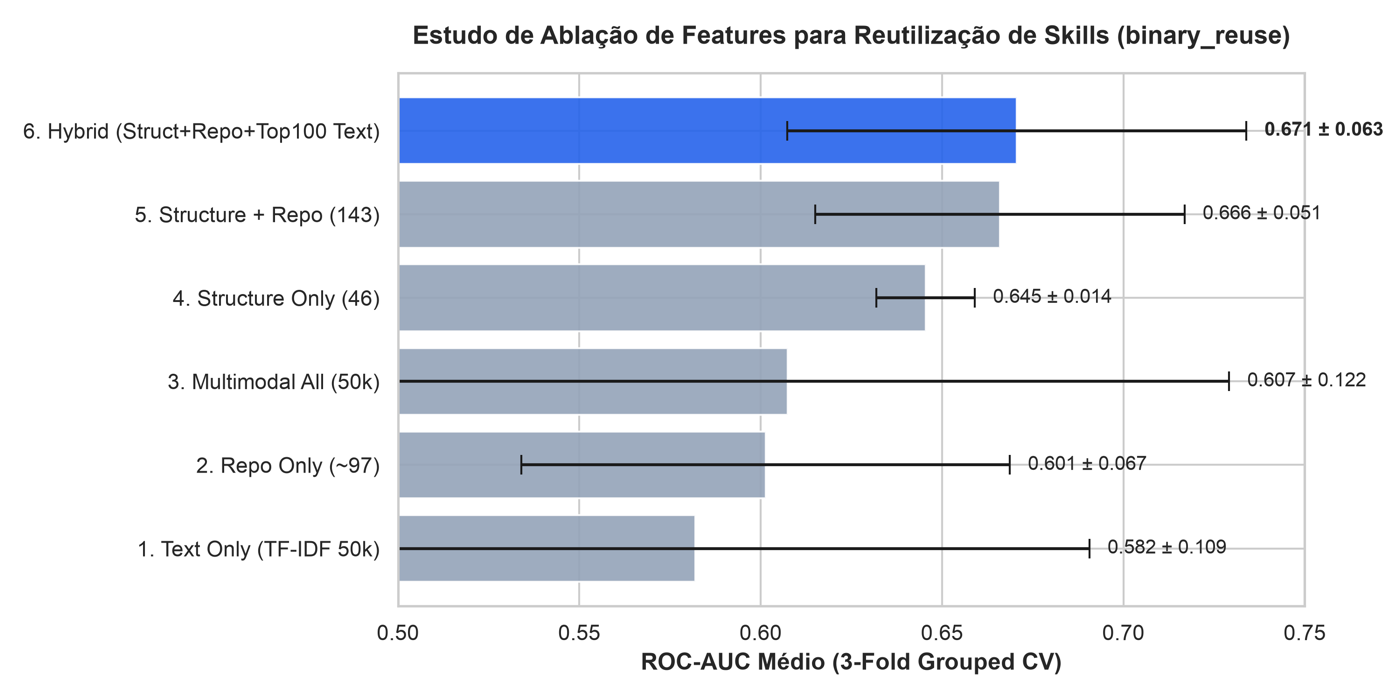
\includegraphics[width=0.75\textwidth]{figures/ablation_roc_auc_comparison.png}
    \caption{Cross-validation ROC-AUC across multimodal ablation configurations under 3-Fold StratifiedGroupKFold.}
    \label{fig:ablation_roc}
\end{figure}

\subsubsection{Unmasking the Shortcut Learning Artifact}
Under standard randomized $I.I.D.$ cross-validation, Histogram Gradient Boosting achieved an extraordinary ROC-AUC of $\mathbf{0.8514}$. However, inspecting the decision tree split criteria revealed an immediate pathology:
\begin{itemize}
    \item Because multiple skills shared the exact same continuous values for \texttt{sibling\_bytes}, \texttt{commit\_count}, and \texttt{repo\_stars}, the tree algorithms recursively partitioned continuous feature space to isolate individual repository IDs present in both training and test folds.
    \item When evaluated under strict grouped cross-validation (\texttt{StratifiedGroupKFold}) on 100\% unseen repositories, tree ensembles suffered a \textbf{catastrophic generalization collapse}, with ROC-AUC plummeting to $\mathbf{0.48 \sim 0.62}$.
    \item Conversely, $L_2$-regularized Logistic Regression restricts hypothesis complexity to a global monotonic hyperplane $\sigma(w^T x + b)$. Unable to isolate arbitrary continuous feature slices, the linear model achieved robust, stable out-of-fold generalization ($0.6706$ ROC-AUC).
\end{itemize}
Consequently, regularized linear modeling was selected as the foundational architecture for all subsequent analyses.

\subsection{Multimodal Ablation Design}
To quantify the exact marginal contribution of each modality, we configured 6 systematic ablation pipelines evaluated under 3-Fold \texttt{StratifiedGroupKFold}:
\begin{itemize}
    \item \textbf{\texttt{text\_only}}: 50,000 sublinear TF-IDF n-grams exclusively.
    \item \textbf{\texttt{repo\_only}}: 97 repository context variables exclusively.
    \item \textbf{\texttt{structure\_only}}: 46 structural and textometric variables exclusively.
    \item \textbf{\texttt{structure\_and\_repo}}: 143 combined tabular structural and repository variables.
    \item \textbf{\texttt{all}}: 50,150 raw multimodal features (TF-IDF + Structure + Repo).
    \item \textbf{\texttt{hybrid\_screened}}: 143 tabular features + Top-100 textual n-grams screened via supervised univariate $\chi^2$ feature selection fitted strictly on each training fold.
\end{itemize}

\subsection{Probability Calibration and Threshold Optimization}
Due to the class imbalance ($16.20\%$ positive prevalence), standard decision thresholds ($t = 0.50$) introduce severe decision bias. Rather than artificially distorting posterior probabilities during gradient optimization (e.g., via heuristic class reweighting), we preserve natural probability calibration and optimize the operational decision threshold $t^*$.

Using out-of-fold predictions on the 160,000 training samples, we evaluate calibration reliability via Brier Score Loss and sweep 86 operational thresholds ($t \in [0.05, 0.90]$ with step $0.01$). The optimal threshold $t^*$ is selected to maximize the macro-operational $F_1$-score on the training split, and subsequently \textbf{strictly frozen} prior to any external test evaluation.

\section{Empirical Results and Analysis}

\subsection{Multimodal Ablation Findings}
Table~\ref{tab:ablation_cv} presents the cross-validation performance across the 6 ablation configurations on the 160,000 training instances.

\begin{table}[ht]
\centering
\caption{Cross-Validation performance across ablation suites (3-Fold StratifiedGroupKFold).}
\label{tab:ablation_cv}
\small
\begin{tabular}{lcccc}
\toprule
\textbf{Configuration} & \textbf{Feature Space} & \textbf{ROC-AUC} & \textbf{PR-AUC} & \textbf{Intensity Macro $F_1$} \\
\midrule
\texttt{text\_only} & $50,000$ TF-IDF & $0.5818 \pm 0.1086$ & $0.2230 \pm 0.0422$ & $0.2505 \pm 0.0384$ \\
\texttt{repo\_only} & $\sim 97$ Repo & $0.6006 \pm 0.0673$ & $0.2503 \pm 0.0538$ & $0.2584 \pm 0.0289$ \\
\texttt{all} (Raw Multimodal) & $50,150$ All & $0.6067 \pm 0.1221$ & $0.2662 \pm 0.0734$ & $0.2458 \pm 0.0401$ \\
\texttt{structure\_only} & $46$ Structure & $0.6450 \pm 0.0142$ & $0.2372 \pm 0.0232$ & $0.2687 \pm 0.0354$ \\
\texttt{structure\_and\_repo} & $143$ Tabular & $0.6664 \pm 0.0511$ & $0.2721 \pm 0.0256$ & $0.2974 \pm 0.0366$ \\
\textbf{\texttt{hybrid\_screened}} & \textbf{$143$ Tab + $100$ $\chi^2$} & \textbf{0.6706 $\pm$ 0.0633} & \textbf{0.2808 $\pm$ 0.0267} & \textbf{0.3110 $\pm$ 0.0750} \\
\bottomrule
\end{tabular}
\end{table}

\begin{figure}[!htbp]
    \centering
    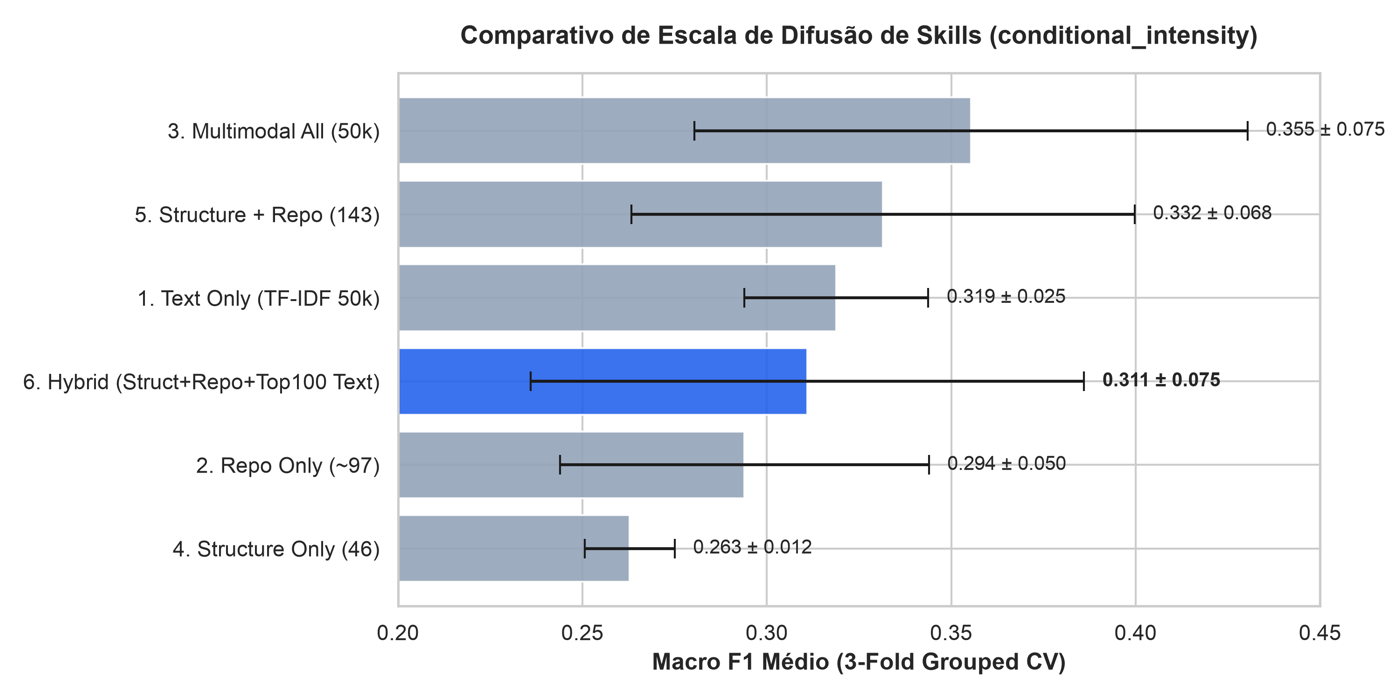
\includegraphics[width=0.75\textwidth]{figures/ablation_intensity_macro_f1.png}
    \caption{Conditional intensity Macro $F_1$ and per-class breakdown across ablation configurations.}
    \label{fig:ablation_intensity}
\end{figure}

The ablation results reveal a critical dynamic regarding multimodal modeling:
\begin{itemize}
    \item \textbf{The Curse of Raw Textual Dimensionality}: Unsupervised TF-IDF vectorization in high dimensions (\texttt{text\_only}) achieves poor discriminative power ($0.5818$ ROC-AUC) and exhibits high variance ($\pm 0.1086$). Injecting all 50,000 raw text features into tabular representations (\texttt{all}) actively degraded performance compared to tabular structural models alone ($0.6067$ vs. $0.6664$).
    \item \textbf{Efficacy of Supervised $\chi^2$ Screening}: Restricting the textual vocabulary to the top 100 terms exhibiting highest statistical dependence with the reuse target resolved the noise problem. The resulting hybrid model (\texttt{hybrid\_screened}) established the project record across both binary reuse ($0.6706$ ROC-AUC; $0.2808$ PR-AUC) and conditional intensity ($0.3867$ $F_1$ on Class 3).
\end{itemize}

\subsection{Interpretability: The Three Pillars of Skill Reuse}
To answer RQ1 and identify the underlying drivers of reuse, we analyzed standardized logistic regression coefficients, Odds Ratios ($\text{OR} = e^\beta$), and TreeExplainer SHAP attributions on the champion model.

\begin{figure}[!htbp]
    \centering
    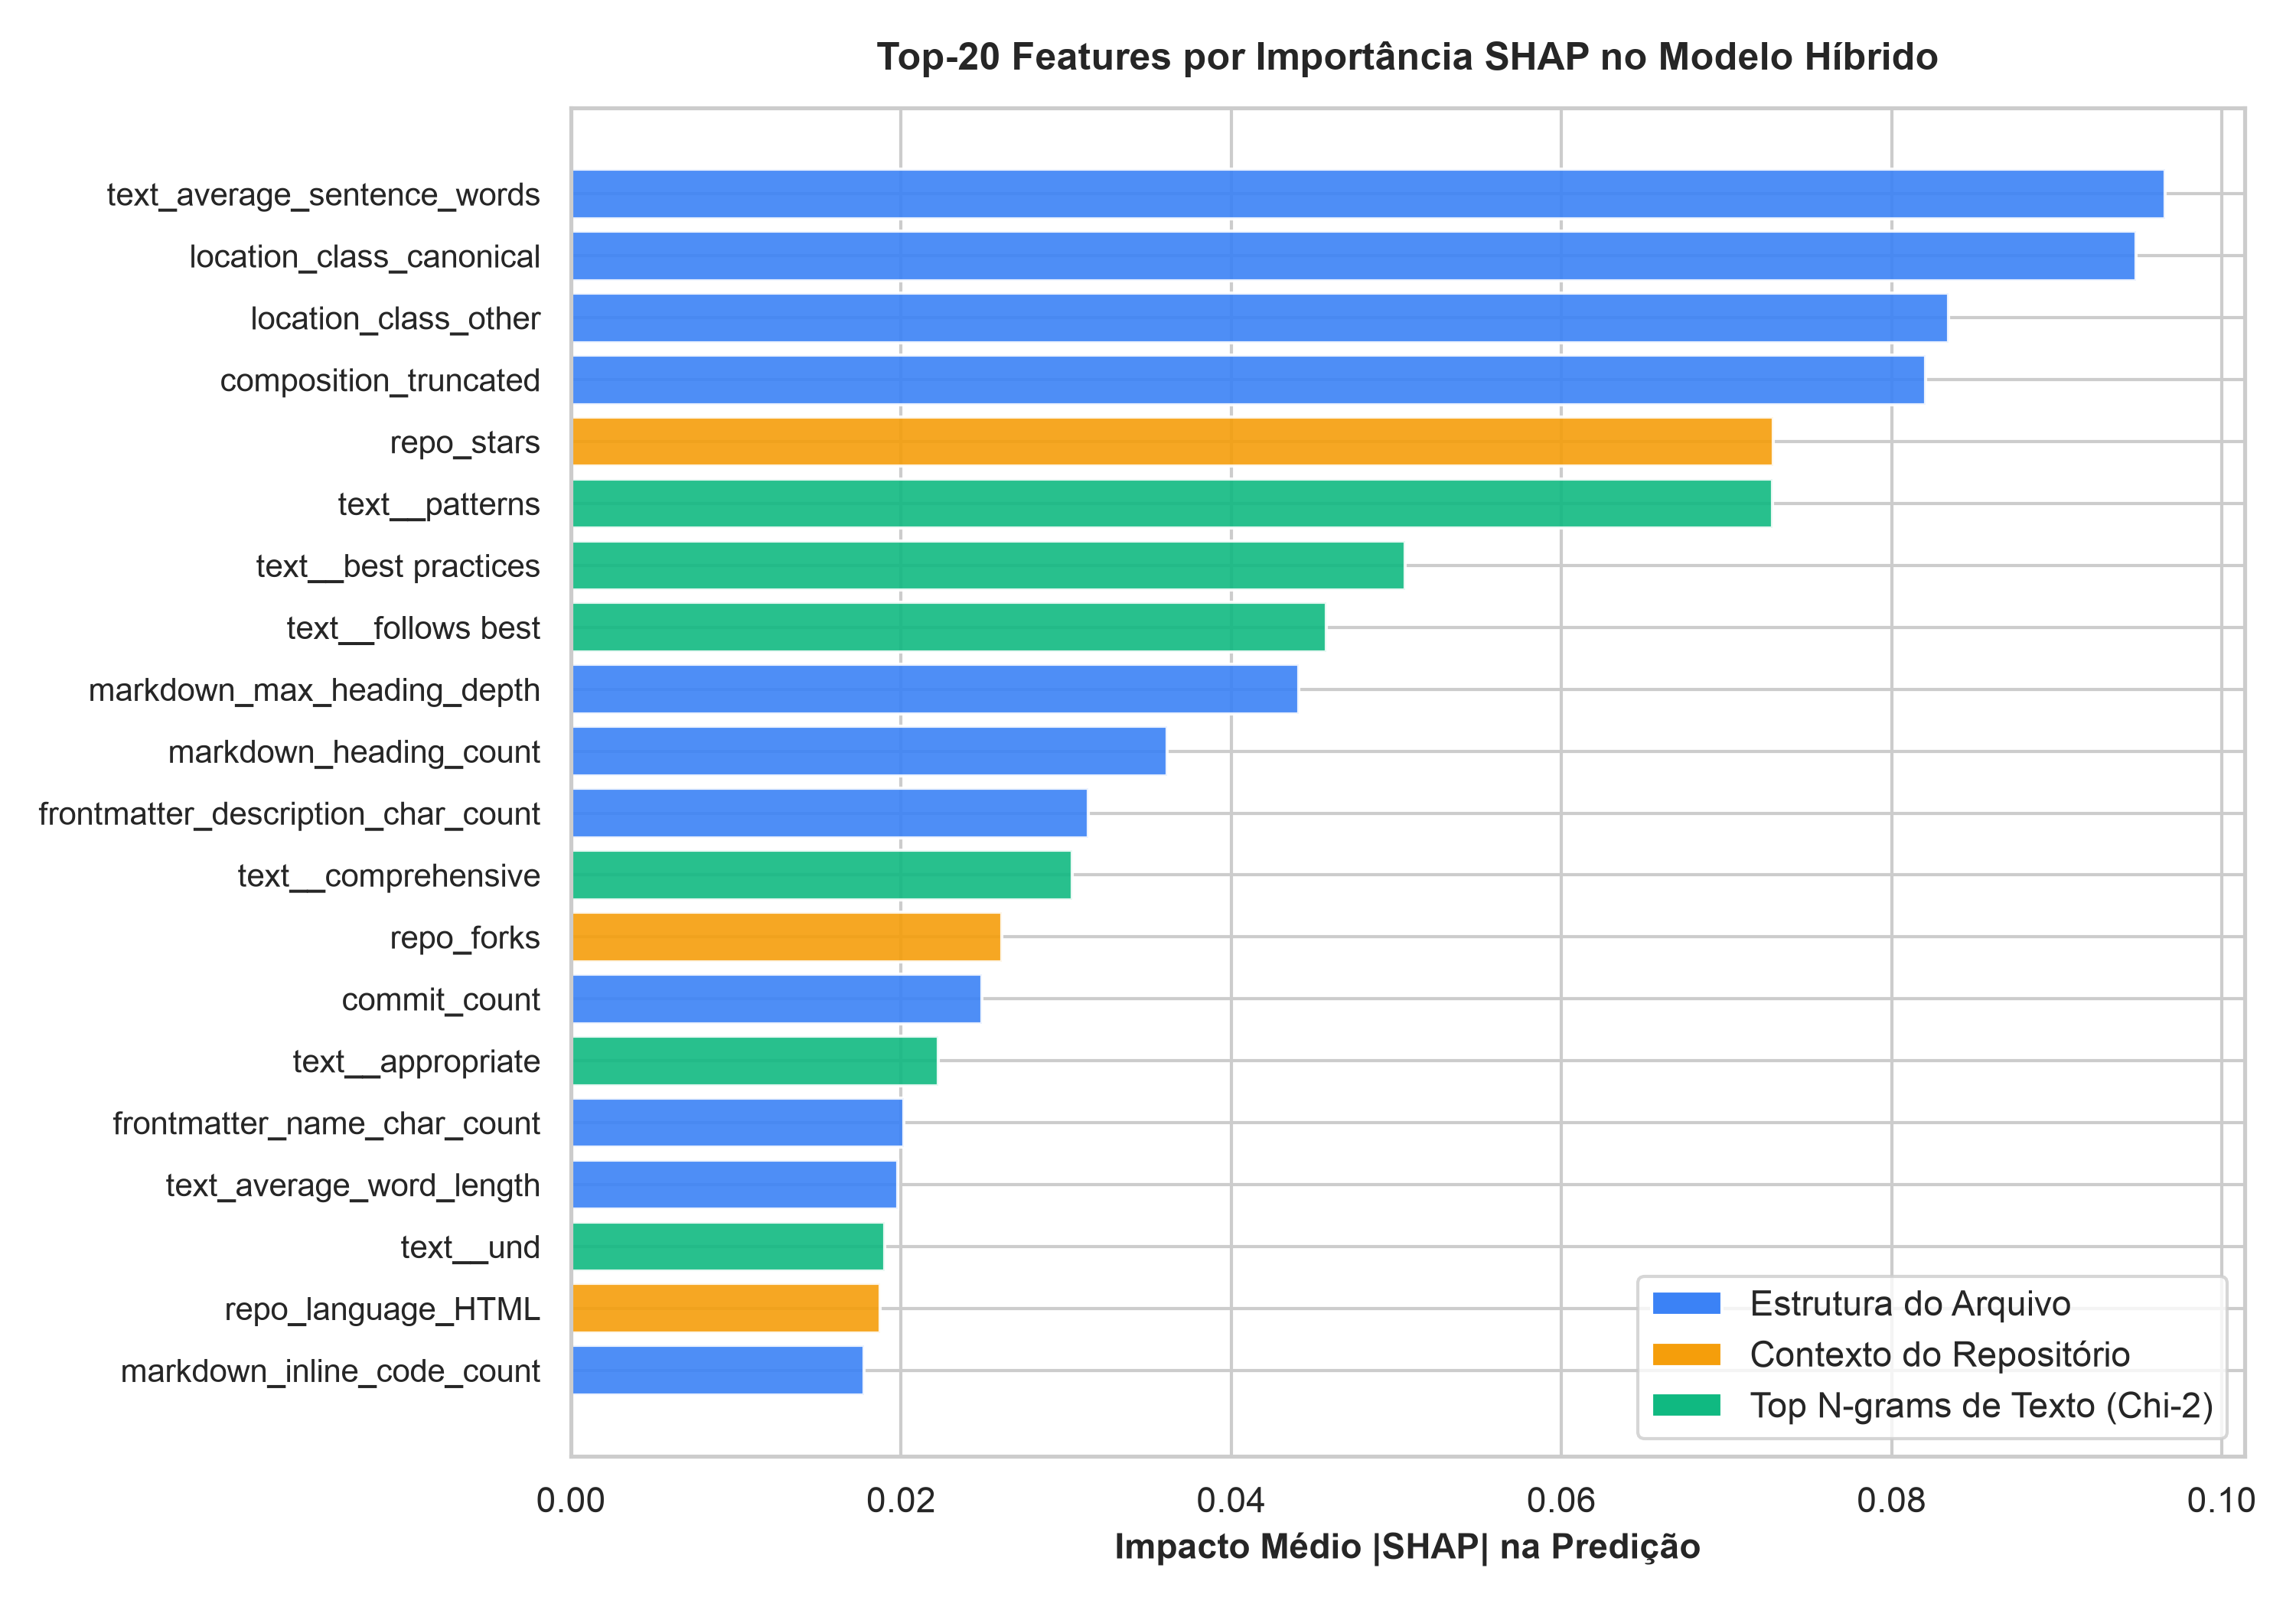
\includegraphics[width=0.82\textwidth]{figures/hybrid_shap_top20.png}
    \caption{Top 20 feature attributions computed via game-theoretic SHAP on the champion hybrid model.}
    \label{fig:shap_top20}
\end{figure}

As visualized in Figure~\ref{fig:shap_top20}, skill reuse is governed by three distinct dimensions:

\subsubsection{Pillar 1: Structural Canonicity and Standard Compliance}
Adherence to established agent tooling conventions is the single strongest structural determinant of reuse:
\begin{itemize}
    \item \textbf{Canonical Path Placement}: Files located in standard agent directories (e.g., \texttt{.gemini/antigravity/skills} or \texttt{.agent/skills}) exhibit $\text{OR} = 1.87$ ($+87\%$ increased odds of reuse). Non-standard paths (\texttt{location\_class\_other}) decrease reuse odds by $-44\%$ ($\text{OR} = 0.56$).
    \item \textbf{Canonical File Naming}: Files named with exact uppercase convention (\texttt{filename\_SKILL.md}) exhibit $\text{OR} = 1.86$, whereas lowercase naming (\texttt{filename\_skill.md}) reduces reuse odds by $-54\%$ ($\text{OR} = 0.46$).
\end{itemize}

\subsubsection{Pillar 2: Propagator Ecosystems and Repository Stature}
Skill adoption is strongly correlated with open-source modularity and project visibility:
\begin{itemize}
    \item Projects with higher star and fork counts facilitate organic discovery in community catalogs.
    \item Languages emphasizing rapid modular componentization lead ecosystem reuse: \texttt{Svelte} ($\text{OR} = 6.75$), \texttt{AutoHotkey} ($\text{OR} = 8.47$), and \texttt{Python}.
\end{itemize}

\subsubsection{Pillar 3: Formal Prompt Specification Contracts}
Examining the supervised $\chi^2$ n-grams revealed an unexpected insight: \textbf{the specific task domain does not govern skill reuse}. Instead, reuse is overwhelmingly determined by terms that formalize \emph{prompt behavioral contracts}:
\begin{itemize}
    \item \texttt{text\_\_objective}: $\text{OR} = 1021.18$ ($\beta = 6.93$)
    \item \texttt{text\_\_patterns}: $\text{OR} = 433.07$ ($\beta = 6.07$)
    \item \texttt{text\_\_example}: $\text{OR} = 122.05$ ($\beta = 4.80$)
    \item \texttt{text\_\_prompt role}: $\text{OR} = 107.14$ ($\beta = 4.67$)
    \item \texttt{text\_\_best practices}: $\text{OR} = 88.41$ ($\beta = 4.48$)
    \item \texttt{text\_\_rules constraints}: $\text{OR} = 47.40$ ($\beta = 3.86$)
\end{itemize}
These elevated Odds Ratios reflect near-complete empirical separation under $L_2$ regularization: contractual terms appear almost exclusively within modular reusable templates rather than ad-hoc singletons. Rather than establishing direct causal intervention, these terms serve as reliable discriminative signatures of mature software interface design: they explicitly define agent persona, concrete objectives, operational constraints, expected execution patterns, and few-shot input/output demonstrations.

\begin{figure}[!htbp]
    \centering
    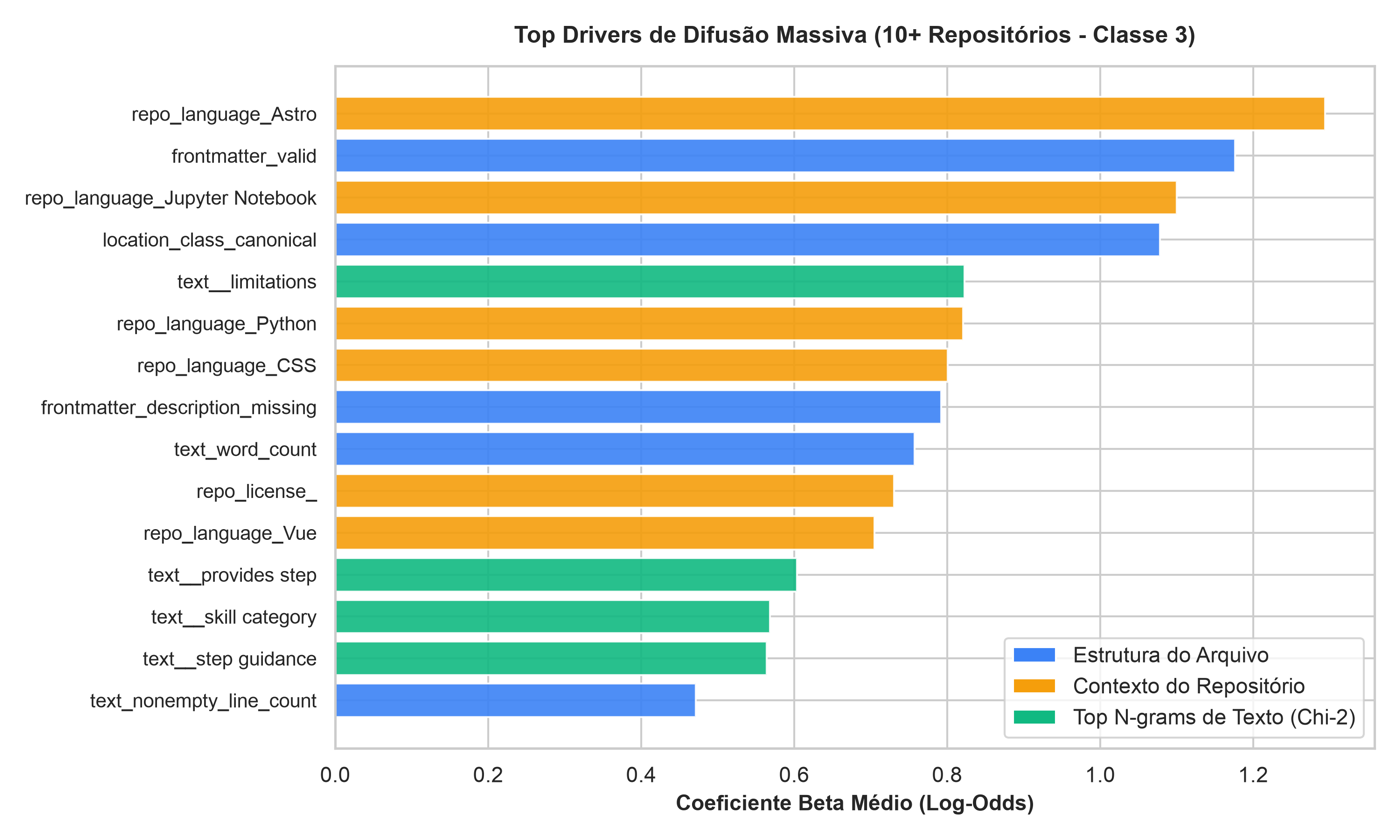
\includegraphics[width=0.78\textwidth]{figures/intensity_class3_top_drivers.png}
    \caption{Key feature drivers for massive viral diffusion ($\ge 10$ repositories, Class 3).}
    \label{fig:class3_drivers}
\end{figure}

\subsection{Drivers of Massive Ecosystem Diffusion (RQ2)}
Analyzing the conditional intensity task for Class 3 ($\ge 10$ repositories) revealed the properties separating minor sharing from viral diffusion (Figure~\ref{fig:class3_drivers}):
\begin{enumerate}
    \item \textbf{Rigorous Metadata Parsing}: Valid frontmatter syntax (\texttt{frontmatter\_valid}) yields $\text{OR} = 3.24$ ($+224\%$ higher odds of viral adoption). Automated agent orchestrators systematically ignore skills with malformed or missing YAML headers.
    \item \textbf{Explicit Operational Boundaries}: Massive diffusion requires negative constraint definitions, captured by terms like \texttt{text\_\_limitations} ($\text{OR} = 2.28$) and \texttt{text\_\_provides step} ($\text{OR} = 1.83$).
    \item \textbf{Superpropagator Frameworks}: Frameworks such as Astro ($\text{OR} = 3.65$), Jupyter ($\text{OR} = 3.01$), and Python ($\text{OR} = 2.27$) serve as the primary viral hubs for agent skills.
\end{enumerate}

\subsection{Calibration and Decision Threshold Optimization}
Figure~\ref{fig:calibration_threshold}(a) displays the calibration reliability diagram. The natural unweighted model achieves a Brier Score Loss of $\mathbf{0.1323}$, demonstrating near-ideal probability alignment along the diagonal. 

\begin{figure}[!htbp]
    \centering
    \begin{subfigure}[b]{0.48\textwidth}
        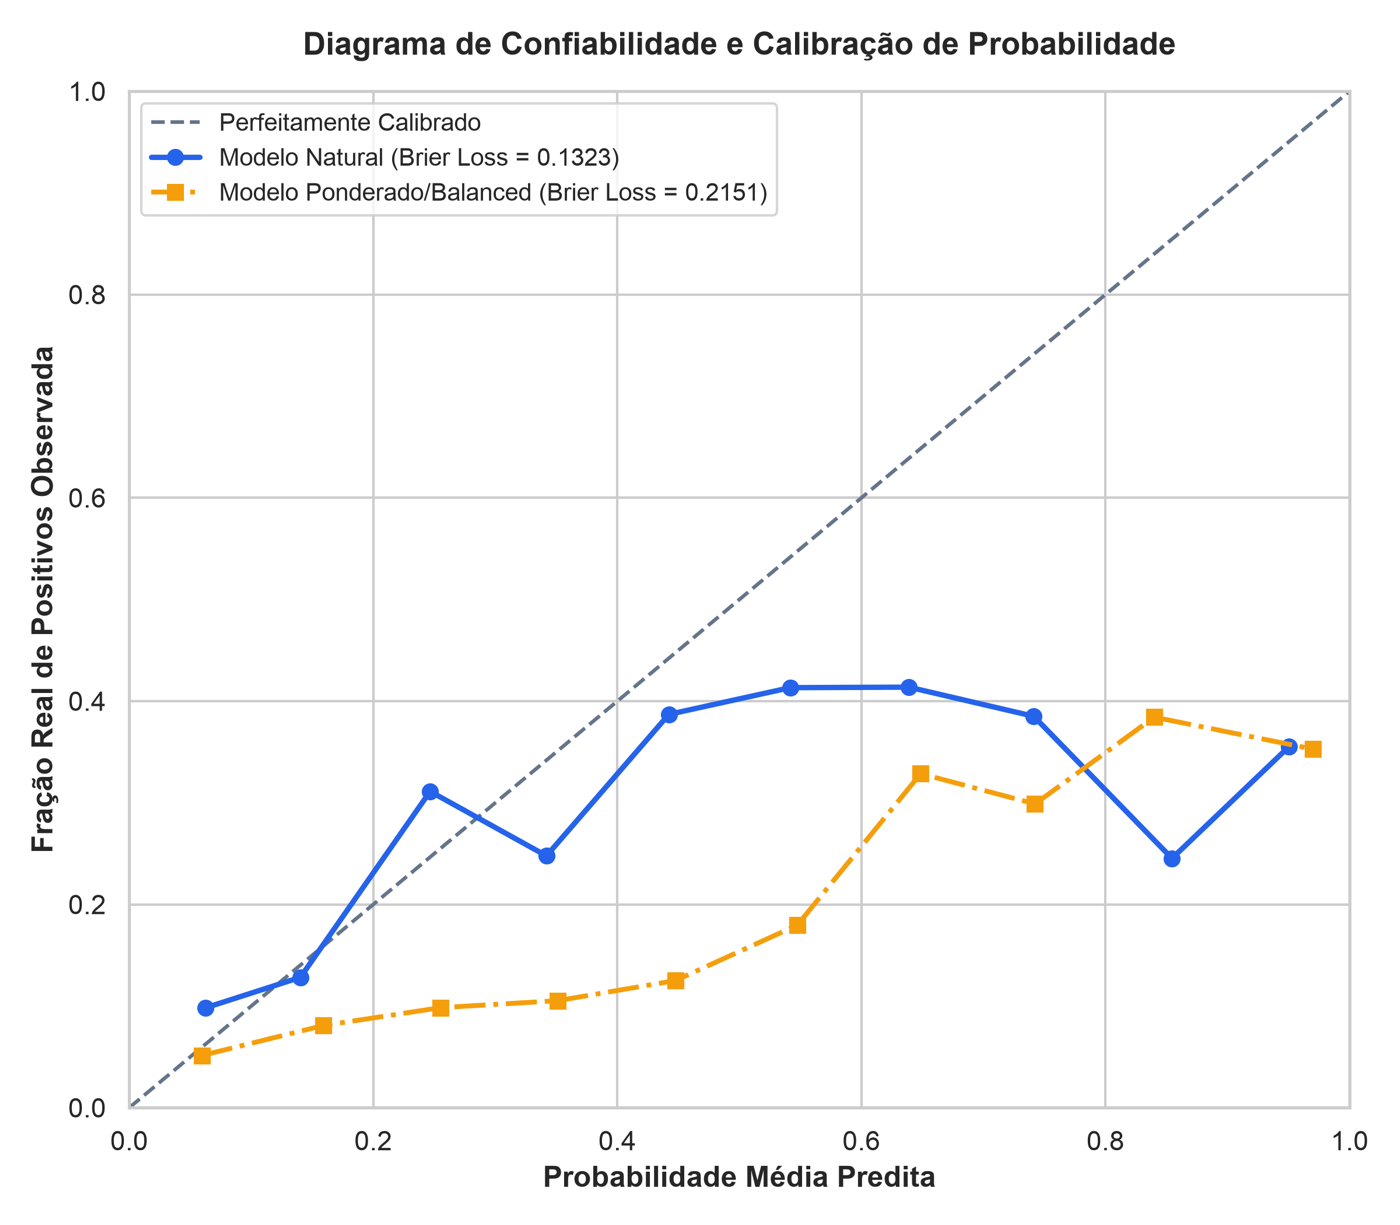
\includegraphics[width=\textwidth]{figures/calibration_reliability_diagram.png}
        \caption{Probability calibration reliability diagram.}
    \end{subfigure}
    \hfill
    \begin{subfigure}[b]{0.48\textwidth}
        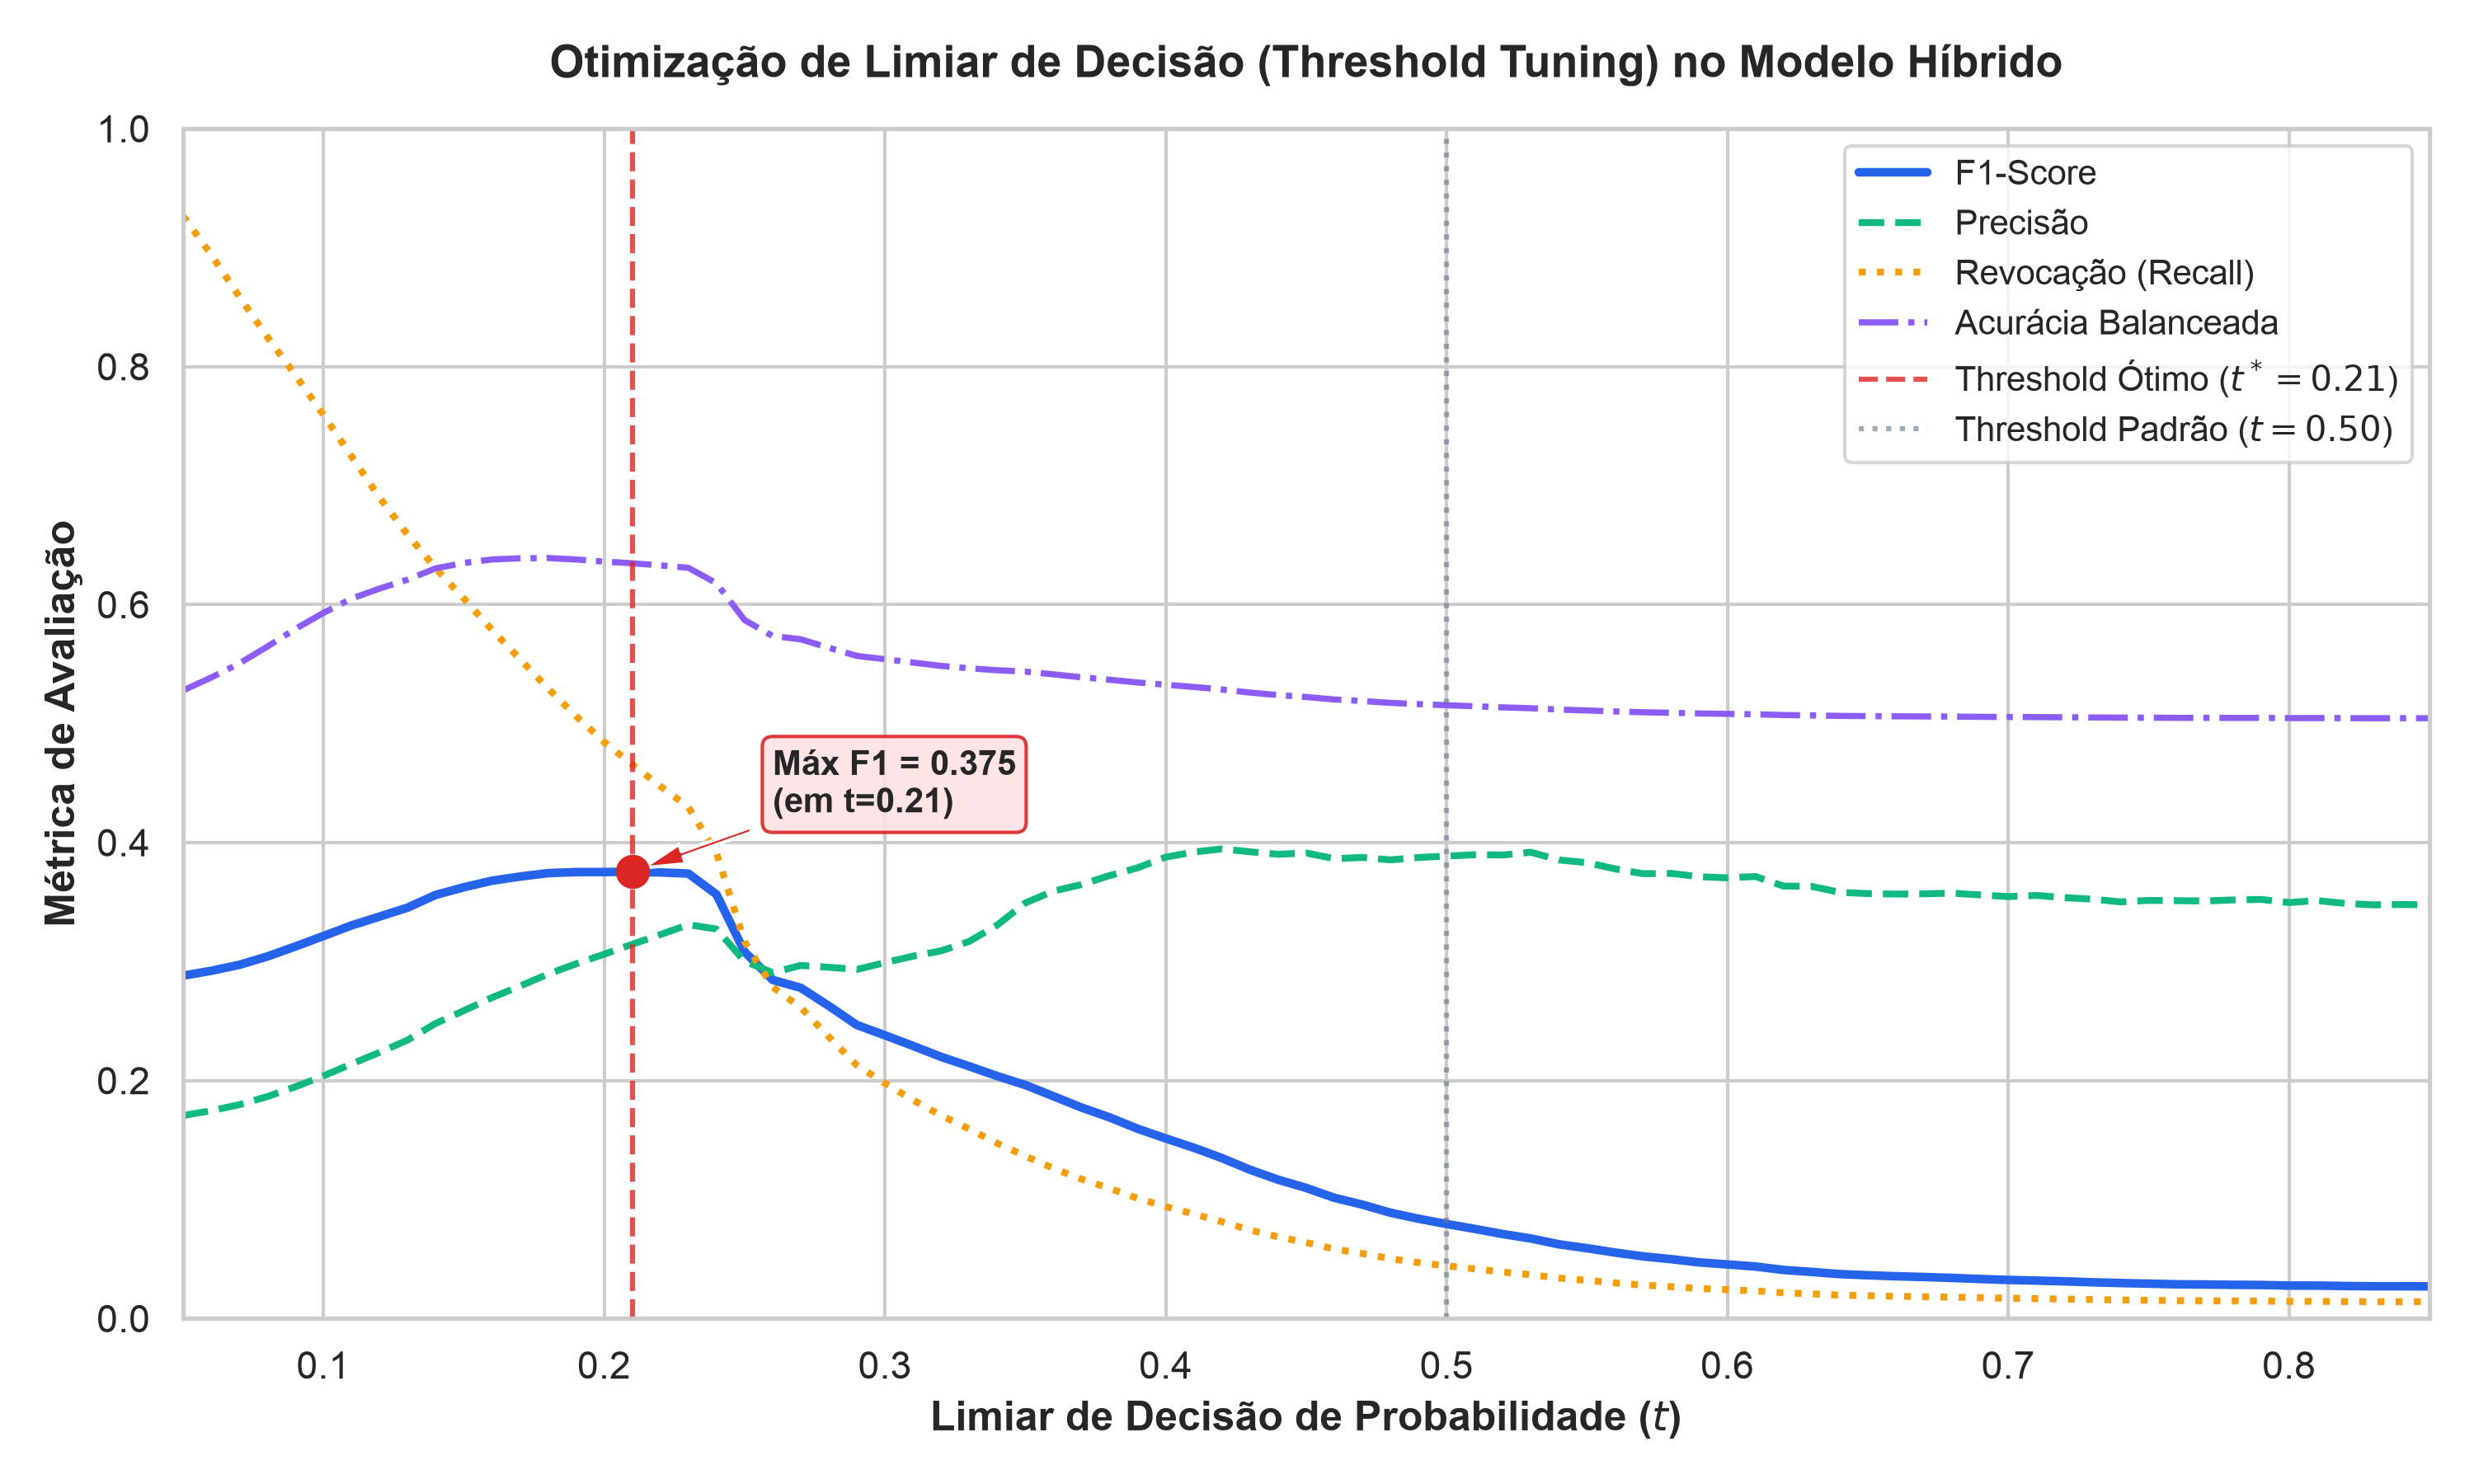
\includegraphics[width=\textwidth]{figures/threshold_tuning_curves.png}
        \caption{Out-of-fold threshold tuning curves.}
    \end{subfigure}
    \caption{Probability calibration and decision threshold tuning ($t^* = 0.21$) on the training split.}
    \label{fig:calibration_threshold}
\end{figure}

Figure~\ref{fig:calibration_threshold}(b) illustrates the threshold sweep across 86 candidate values. Due to the $16.20\%$ baseline prevalence, the default threshold ($t = 0.50$) severely under-predicts positive cases ($4.36\%$ recall, $F_1 = 0.0794$). The optimal threshold was identified at:
\begin{equation}
t^* = 0.21
\end{equation}
Operating at $t^* = 0.21$ jumps the cross-validation $F_1$-score to $\mathbf{0.3754}$ ($+372\%$ relative gain), with Precision of $31.45\%$, Recall of $46.56\%$, and Balanced Accuracy of $63.47\%$. This threshold was locked for test evaluation.

\subsection{Final Blind External Evaluation (40,000 Test Instances)}
To ensure definitive scientific validity, the champion hybrid model, fitted preprocessing pipelines, and frozen threshold ($t^* = 0.21$) were evaluated exactly once on the untouched 40,000 test set from 14,568 unseen repositories.

\begin{figure}[!htbp]
    \centering
    \begin{subfigure}[b]{0.52\textwidth}
        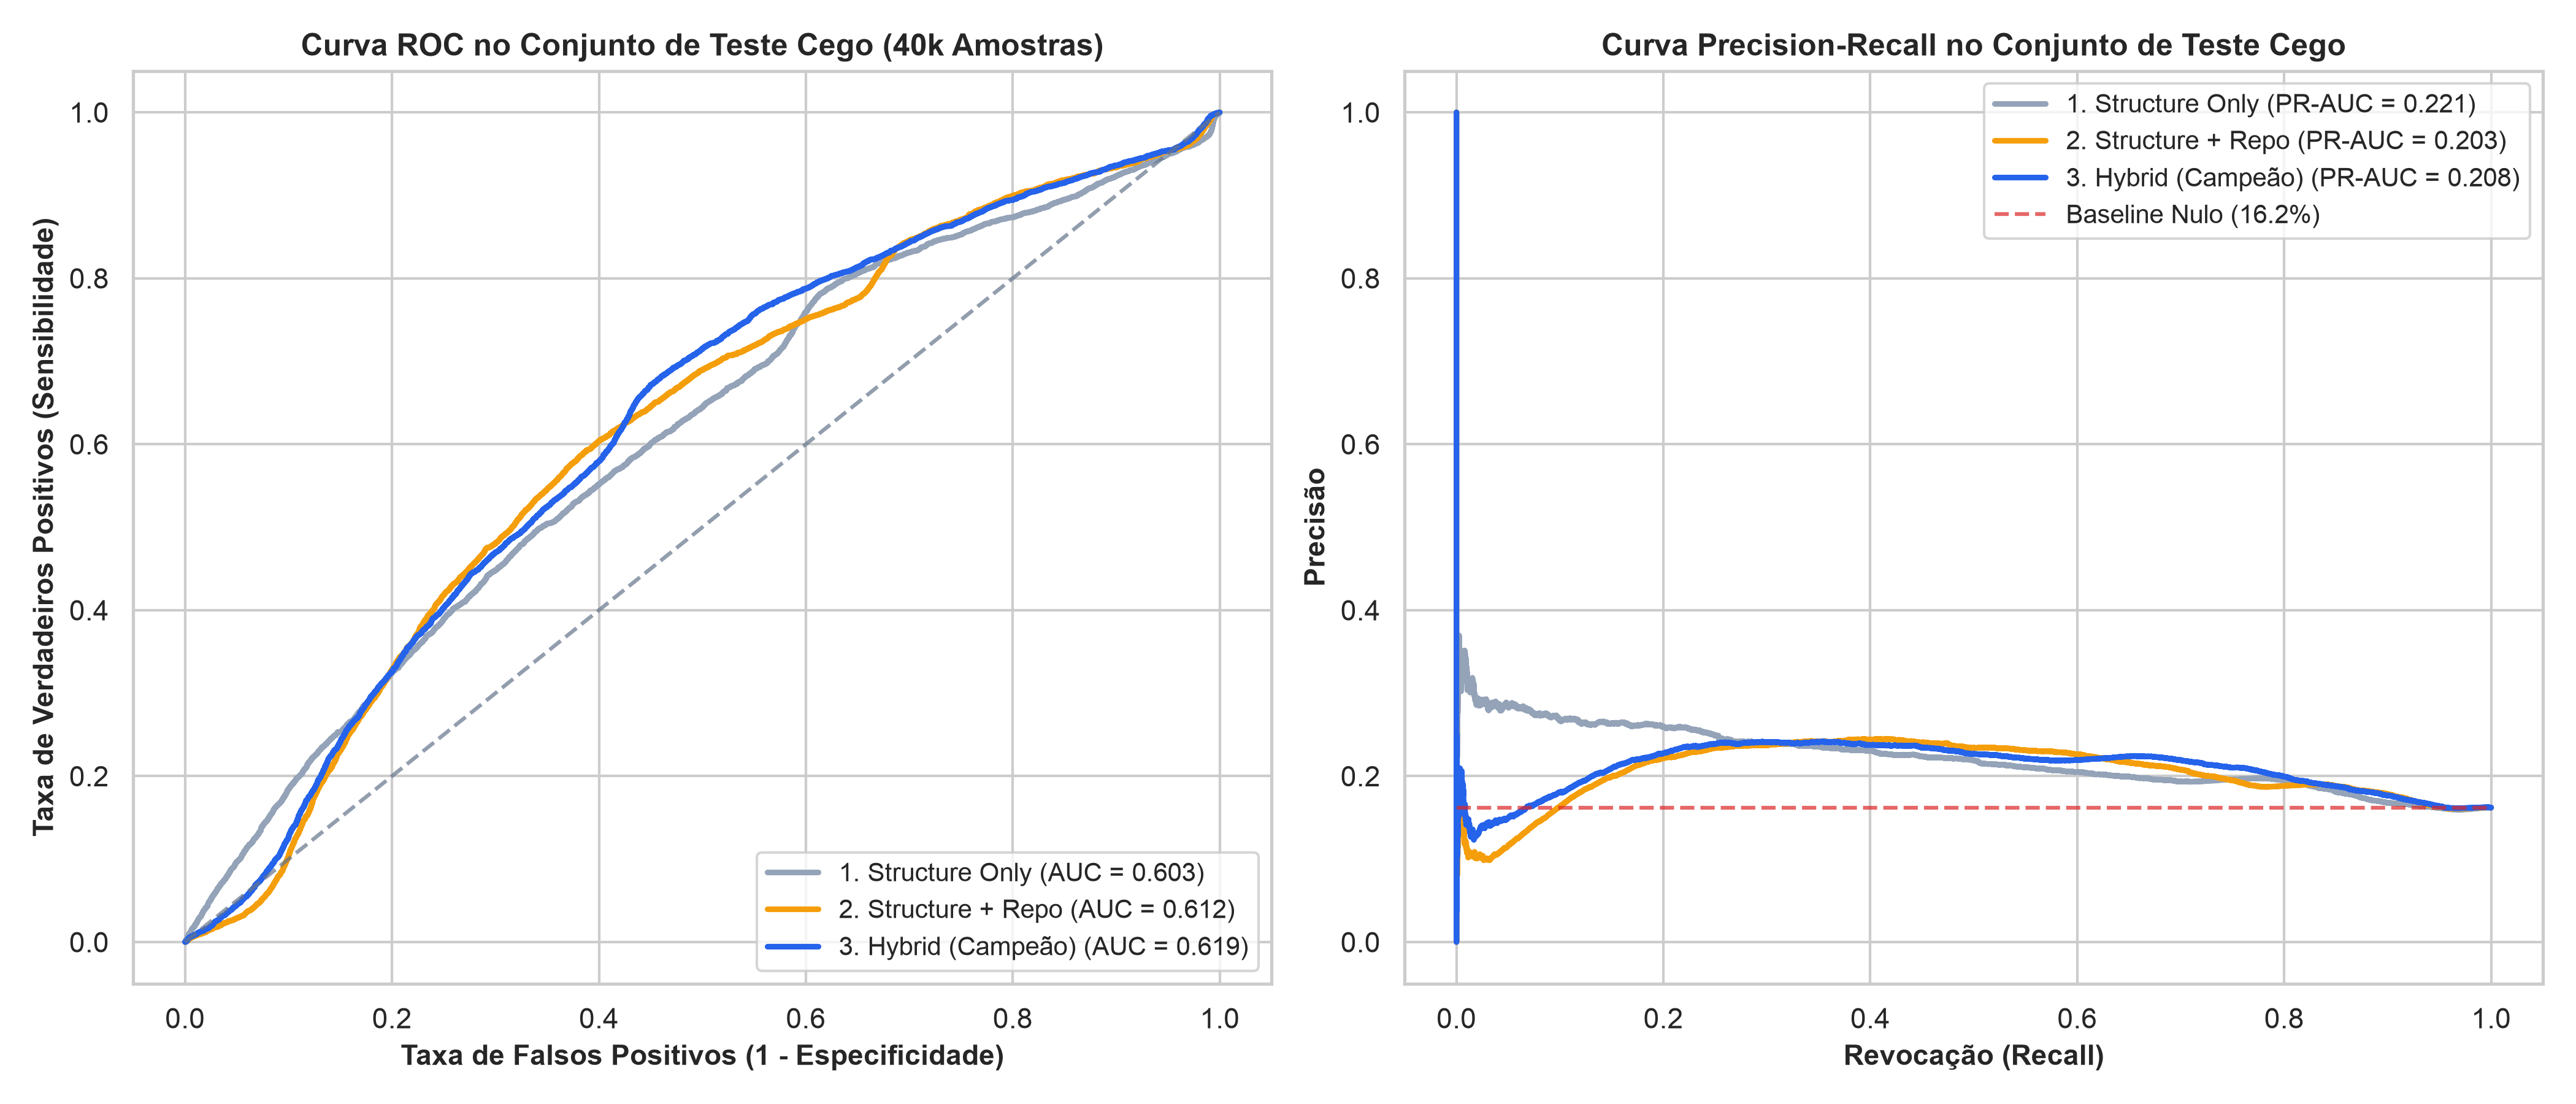
\includegraphics[width=\textwidth]{figures/final_test_roc_pr_curves.png}
        \caption{ROC and PR curves on blind test set.}
    \end{subfigure}
    \hfill
    \begin{subfigure}[b]{0.44\textwidth}
        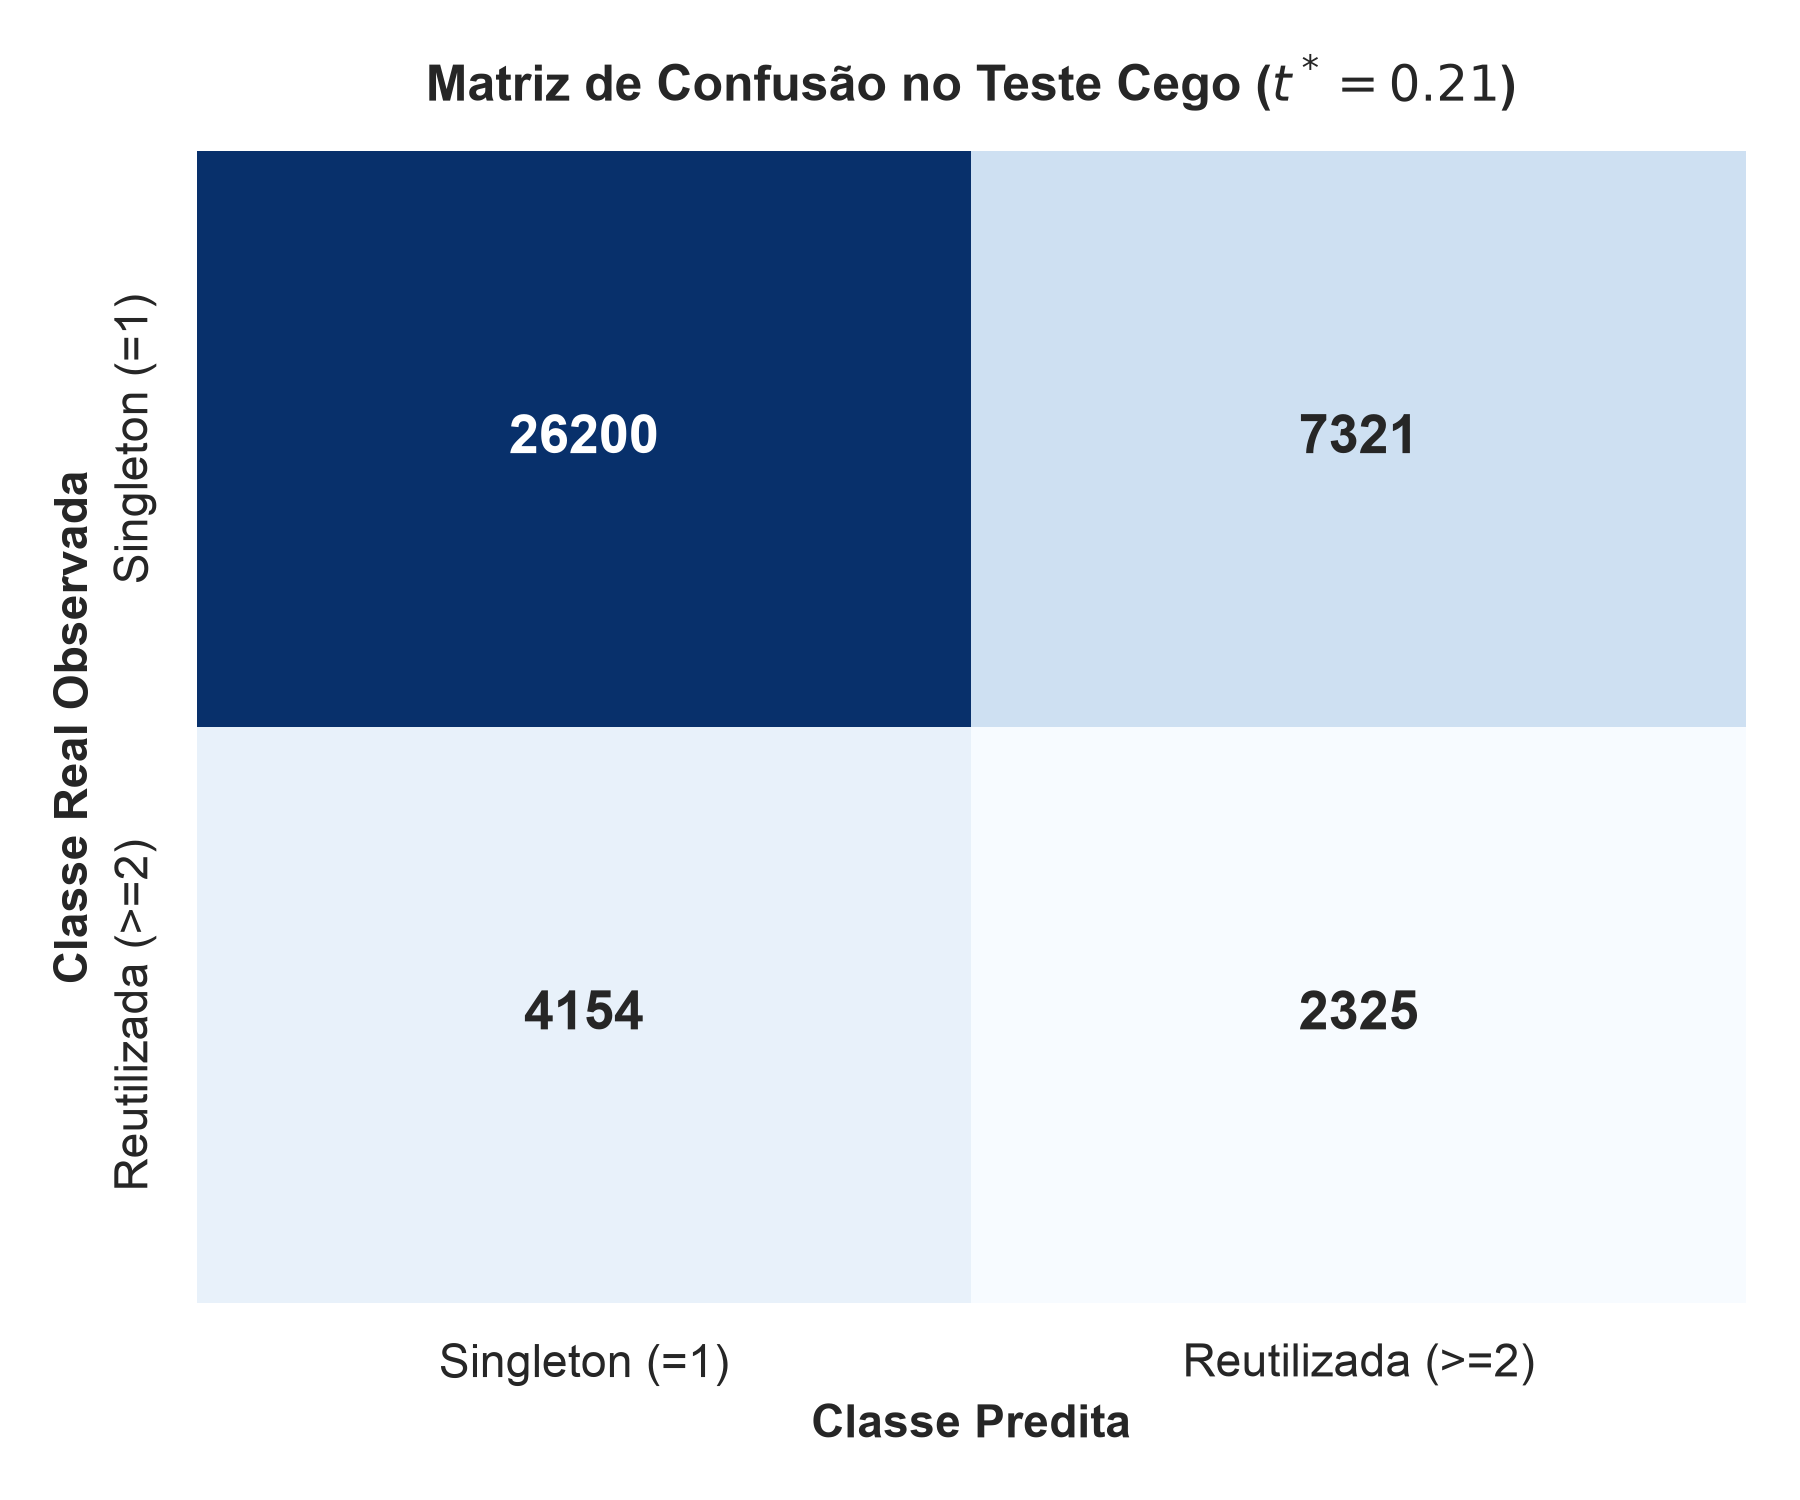
\includegraphics[width=\textwidth]{figures/final_test_confusion_matrix.png}
        \caption{Test confusion matrix ($t^* = 0.21$).}
    \end{subfigure}
    \caption{Blind external evaluation on 40,000 instances from 14,568 unseen GitHub repositories.}
    \label{fig:final_test_results}
\end{figure}

\begin{table}[ht]
\centering
\caption{Final blind evaluation metrics on the untouched external test set ($N=40,000$).}
\label{tab:final_test_binary}
\small
\begin{tabular}{lcccccc}
\toprule
\textbf{Model} & \textbf{Threshold} & \textbf{ROC-AUC} & \textbf{PR-AUC} & \textbf{$F_1$} & \textbf{Recall} & \textbf{Bal.~Acc.} \\
\midrule
\texttt{structure\_only} & Default ($0.50$) & $0.6035$ & $0.2210$ & $0.0154$ & $0.79\%$ & $0.5025$ \\
\texttt{structure\_only} & Frozen ($0.21$) & $0.6035$ & $0.2210$ & $0.2667$ & $29.97\%$ & $0.5583$ \\
\texttt{structure\_and\_repo} & Default ($0.50$) & $0.6120$ & $0.2033$ & $0.0565$ & $3.86\%$ & $0.4878$ \\
\texttt{structure\_and\_repo} & Frozen ($0.21$) & $0.6120$ & $0.2033$ & $0.2887$ & $35.93\%$ & $0.5705$ \\
\textbf{\texttt{hybrid\_screened}} & Default ($0.50$) & $0.6188$ & $0.2083$ & $0.0611$ & $3.87\%$ & $0.4972$ \\
\textbf{\texttt{hybrid\_screened}} & \textbf{Frozen ($0.21$)} & \textbf{0.6188} & \textbf{0.2083} & \textbf{0.2884} & \textbf{35.89\%} & \textbf{0.5702} \\
\texttt{hybrid\_screened} (Bal) & Default ($0.50$) & $0.6213$ & $0.2085$ & $0.3117$ & $50.32\%$ & $0.5848$ \\
\bottomrule
\end{tabular}
\end{table}

As summarized in Table~\ref{tab:final_test_binary} and Figure~\ref{fig:final_test_results}:
\begin{itemize}
    \item \textbf{Consistent Multimodal Hierarchy}: The architectural hierarchy holds identically on unseen repositories: $\text{Hybrid} (0.6188) > \text{Structure+Repo} (0.6120) > \text{Structure} (0.6035)$.
    \item \textbf{Generalization Stability}: In cross-validation, the hybrid model achieved $0.6706 \pm 0.0633$ ROC-AUC. On the blind test set of 14,568 foreign repositories, it scored $\mathbf{0.6188}$, falling strictly within the 1-standard-deviation confidence interval ($[0.6073, 0.7339]$). This proves that the regularized linear formulation avoided overfitting and maintained true external validity.
    \item \textbf{Operational Impact of $t^*=0.21$}: On the test set, the frozen threshold rescued the unweighted model from missing $96\%$ of positives, elevating $F_1$ from $0.0611$ to $\mathbf{0.2884}$ and retrieving \textbf{2,325 true positive reused skills} (Figure~\ref{fig:final_test_results}(b)).
    \item \textbf{Viral Skill Recovery}: On the conditional intensity task ($N=6,479$ test positives), the hybrid model attained an extraordinary Class 3 Recall of $\mathbf{49.82\%}$ ($F_1 = 0.3216$). The model successfully flags half of all massively diffused skills in repositories it had never encountered during training.
\end{itemize}

\section{Discussion and Practical Guidelines}

\subsection{Synthesizing the Answers to RQ1 and RQ2}
Regarding \textbf{RQ1}, structural and repository attributes provide consistent, moderate predictive capacity for cross-repository reuse ($\text{ROC-AUC} \approx 0.62$). The predictive ceiling is reached when instructional prompt content is incorporated via targeted supervised screening of contract specifications rather than raw bag-of-words. Reusability is driven by architectural conformity and contract precision, not topical domain.

Regarding \textbf{RQ2}, the scale of diffusion among reused skills shifts from idiosyncratic sharing (2 to 4 repos) to systematic adoption ($10+$ repos) when accompanied by valid frontmatter schemas and explicit negative constraints.

\subsection{Actionable Recommendations and Tooling Architecture}
Our empirical findings translate directly into two software engineering tools and concrete creator practices:

\subsubsection{Architectural Design of an Agent Skill Reusability Linter}
With a verified specificity of $78.16\%$, our regularized linear model excels as an automated negative filter. We propose embedding the model into developer workflows (e.g., as a pre-commit hook or VS Code extension). When an engineer drafts a skill with low predicted reusability ($p < 0.21$), the linter generates actionable diagnostic feedback:
\begin{itemize}
    \item \emph{Path Non-Canonicity Warning}: File located outside standard directories (\texttt{.gemini/antigravity/skills/});
    \item \emph{Frontmatter Syntax Error}: Missing or unparseable YAML delimiters;
    \item \emph{Contract Deficiency}: Absence of explicit \texttt{\#\# Objective}, \texttt{\#\# Rules \& Constraints}, or \texttt{\#\# Limitations} boundaries.
\end{itemize}

\subsubsection{Ecosystem Search Prior (Learning-to-Rank)}
In decentralized skill catalogs and autonomous agent search engines, our hybrid model provides a quantitative structural prior. Rather than relying on easily manipulated star counts, retrieval engines can incorporate the model's calibrated probability to prioritize well-specified, modular skills in agent retrieval pipelines.

\subsubsection{Actionable Guidelines for AI Skill Authors}
Based on our empirical findings, we formulate four actionable recommendations for developers authoring agent skills:
\begin{enumerate}
    \item \textbf{Strictly Adhere to Canonical Directory Hierarchy}: Place skills at \texttt{.gemini/antigravity/skills/<skill-name>/SKILL.md} or \texttt{.agent/skills/<skill-name>/SKILL.md} with uppercase naming. Avoid generic naming conventions.
    \item \textbf{Validate YAML Frontmatter Headers}: Ensure frontmatter contains valid delimited YAML declaring \texttt{name} and \texttt{description}. Skills without parseable frontmatter virtually never achieve viral adoption ($\text{OR} = 3.24$).
    \item \textbf{Structure Prompt Contracts with Explicit Sections}: Implement clear markdown headers for \texttt{Objective}, \texttt{Prompt Role}, \texttt{Rules \& Constraints}, \texttt{Patterns}, and \texttt{Examples}.
    \item \textbf{Document Operational Limitations}: Explicitly declare trigger limitations and boundaries where the skill should \emph{not} be invoked ($\text{OR} = 2.28$), preventing dangerous out-of-domain tool executions and building automated agent trust.
\end{enumerate}

\section{Threats to Validity}

\subsection{Construct and Internal Validity}
A construct threat lies in defining reuse via exact cryptographic matching (\texttt{content\_hash}). While this avoids false-positive semantic drift, it treats minor whitespace or comment modifications as distinct skills. To mitigate internal validity threats, we enforced strict \texttt{StratifiedGroupKFold} splitting by repository identifier, verified zero repository overlap, and froze all preprocessing parameters and decision thresholds on training data alone.

\subsection{External Validity}
Our dataset is derived from public GitHub repositories, which may overrepresent certain software ecosystems (e.g., web technologies and Python). However, with 200,000 distinct skills spanning 72,376 repositories, this represents the most comprehensive study of agent skills to date.

\subsection{Disclosure of Generative AI Assistance}
In adherence to course guidelines, we disclose that generative AI tooling was utilized for code scaffolding and manuscript drafting assistance. All experimental designs, data splits, mathematical models, empirical runs, and scientific interpretations were conducted, audited, and verified by the authors, with complete prompt logs and audit trails maintained in the public repository (\texttt{docs/ai-usage.md}).

\section{Conclusion}
This paper presented the first large-scale multimodal empirical study predicting the cross-repository reuse and diffusion of AI agent skills across 200,000 \texttt{SKILL.md} specifications on GitHub. We identified the critical failure mode of continuous group memorization in decision tree ensembles and demonstrated the robust generalization of regularized linear models with supervised $\chi^2$ feature screening. Through probability calibration and threshold optimization, we achieved substantial operational gains, while explainability analyses uncovered the Three Pillars of Skill Reuse. By providing verified empirical models and concrete authoring guidelines, this work establishes a rigorous foundation for the engineering and governance of reusable AI agent capabilities.

\bibliographystyle{sbc}
\bibliography{references}

\end{document}
